% REMEMBER: You must not plagiarise anything in your report. Be extremely careful.

\documentclass{l4proj}
\usepackage{placeins}
\setcitestyle{square}




    
%
% put any additional packages here
%

\begin{document}

%==============================================================================
%% METADATA
\title{Hybrid Localization with video based positioning technology}
\author{Tan De Hui Adrian}
\date{October 3, 2019 - first date}

\maketitle

%==============================================================================
%% ABSTRACT
\begin{abstract}
     Global Positioning Systems (GPS) have revolutionised technology and are used in nearly every aspect of life in today's world. However, the application of the 		underlying technology in GPS does not solve the problems of indoor localization. Indoor localization has recently witnessed an increase in interest, due to the potential wide range of services it can provide by leveraging Internet of Things (IoT) and ubiquitous connectivity. Many different techniques such as the use of WiFi, Radio Frequency Identification Systems and others have been utilised to fix such problems. These technologies are expensive in nature due to the demands for additional infrastructure to be installed, leading to high budget and labor cost. In this paper, we have proposed the solution of using QR Code in conjunction with Inertial Measurement Unit (IMU). IMU includes sensors such as accelerometers and gyroscopes which can lead to a cumulative error over time. QR Code will then aid in reducing the cumulative error. This paper presents an effective way for indoor navigation using inertial measurement unit (IMU) in conjunction with a quick response (QR) code. Usage of QR codes helps to compensate the errors from the IMU thereby providing accurate navigation. This technique involves very less cost and can be implemented in a straight forward manner.  -- add result in.
\end{abstract}

%==============================================================================

% EDUCATION REUSE CONSENT FORM
% If you consent to your project being shown to future students for educational purposes
% then insert your name and the date below to  sign the education use form that appears in the front of the document. 
% You must explicitly give consent if you wish to do so.
% If you sign, your project may be included in the Hall of Fame if it scores particularly highly.
%
% Please note that you are under no obligation to sign 
% this declaration, but doing so would help future students.
%
%\def\consentname {My Name} % your full name
%\def\consentdate {20 March 2018} % the date you agree
%
\educationalconsent


%==============================================================================
\tableofcontents

%==============================================================================
%% Notes on formatting
%==============================================================================
% The first page, abstract and table of contents are numbered using Roman numerals and are not
% included in the page count. 
%
% From now on pages are numbered
% using Arabic numerals. Therefore, immediately after the first call to \chapter we need the call
% \pagenumbering{arabic} and this should be called once only in the document. 
%
% The first Chapter should then be on page 1. You are allowed 40 pages for a 40 credit project and 20 pages for a 
% 20 credit report. This includes everything numbered in Arabic numerals (excluding front matter) up
% to but excluding the appendices and bibliography.
%
% You must not alter text size (it is currently 10pt) or alter margins or spacing.
%
%
%==================================================================================================================================
%
% IMPORTANT
% The chapter headings here are **suggestions**. You don't have to follow this model if
% it doesn't fit your project. Every project should have an introduction and conclusion,
% however. 
%
%==================================================================================================================================
\chapter{Introduction}

% reset page numbering. Don't remove this!
\pagenumbering{arabic} 

\section{Indoor localization}
In current day, location-based services (LBS) have become an important part of people’s daily lives. Demands for LBS in indoor environments have also increased for purposes like indoor path finding and navigation, marketing, entertainment and location-based information retrieval. Many technologies have been utilised for LBS in indoor however many are inaccurate.\\

Smartphones in the current generation has become increasingly powerful and advanced, especially its built-in sensors, wireless technologies and processor computing power. Hence, many users are making use of such advanced and power technologies embedded on their smartphone to perform many different functionalities.\\

One main application that users are using on their smartphone is the LBS for outdoor navigation. Such applications have been developed using the global positioning system (GPS) which provides the users with geographical information, street view and different kinds of maps. Such services have been asked to be replicated for an indoor environment. However, such approaches used in outdoor based location services cannot be applied to indoor based as the signal reception indoor is limited in indoor environment such as in buildings, tunnels etc. This often leads to poor or inaccurate position within the building being reflected to the users.\\

\section{Measures taken for Indoor Positioning Systems}
In order to address such challenges posed from the GPS in indoor environment, many different technologies have been studied and utilised to be applicable for indoor based location services. Instead of using GPS, some technologies studied for indoor based location services are the use of Wi-Fi, Bluetooth Low Energy (BLE) Beacon, Ultra-Wide Band (UWB), Ultrasonic wave, Radio Frequency Identification (RFID), Geomagnetic field and Inertial Measurement Unit (IMU). [R. Harle, A survey of indoor inertial positioning systems for pedestrians. IEEE Communications Surveys &
447 Tutorials, vol. 15, no. 3, pp. 1281-–1293, 2013.][ W. Sakpere, M. Adeyeye Oshin, and N. B. Mlitwa, A State-of-the-Art Survey of Indoor Positioning and
449 Navigation Systems and Technologies. South African Computer Journal, vol. 29, no. 3, pp. 145-–197, 2017.
450 3. G. Deak, K. Curran, and J. Condell, A survey of active and passive indoor localisation systems. Computer
451 Communications, vol. 35, no. 16, pp. 1939—1954, 2012.] These listed technologies can perform personal indoor navigation, marketing, location-based entertainment, indoor emergency localization and many others. With such technologies being actively utilised in several aspects for the individual users, the technologies must be able to provide reasonably accurate positioning data for the different type of indoor positioning application.\\

The most commonly studied technologies for the indoor positioning systems (IPS) are Wi-Fi and Bluetooth beacons as these two technologies are much more readily available than other technologies – with wireless access points being installed in many common areas and Bluetooth access in the common areas as well. The Wi-Fi and Bluetooth positioning method mainly focus on time of Arrival (ToA), angle of arrival (AoA) and Received Signal Strength Indicator (RSSI), with RSSI based positioning system the most widely implemented due to its reasonably acceptable indoor positioning accuracy. However, this method heavily depends on the stability of the RSSI as well as the line of sight between the transmitter and receiver devices.\\

Another popular implementation is the IMU sensor, consisting of accelerometer, gyroscope and magnetometers. The implementation of such IMU sensors are relatively low cost and the pedestrian dead reckoning positioning algorithm does not require any additional installation of infrastructure. However, the use of this method only allows for a reasonable accuracy for a short distance as it suffers from a cumulative error, leading to a drift in heading estimation over time. This drift error will also accumulate over time while utilising low cost IMU sensors embedded in the smartphone but can be handled with heading drift reduction techniques. Integration of other technologies in conjunction with IMU sensors can help to mitigate the drift error brought about by the IMU sensors from the smartphone.\\

\section{Discussion in this paper}
In this paper, an application using the smartphone’s embedded IMU sensors together with Quick Response (QR) Code is developed for indoor positioning. The QR code will contain the coordinates that helps to reset the indoor position of the user holding on the smartphone in order to counter the heading drift. It will also effectively tell how far the user is away from the QR code.


\chapter{Literature Review}
\section{Overview}
Location-based services (LBS) is now an essential and integral part of individual's everyday work and life in recent years. The Global Navigation Satellite System (GNSS) plays an important role in LBS and the various enhancement technologies can make GNSS achieve sub meter positioning accuracy in an open area. \cite{yzhuang} However the capability of GNSS in and outdoor environment cannot be replicated in an indoor environment as it is not possible to be able to guarantee the availbility of the satellite signals that GNSS make use of for navigation. In order to counter such problems faced in an indoor environment, many other approaches have been extensively studied upon to enhance Indoor Positioning System (IPS) such as wireless local area network (WLAN) \cite{yzhuang}, ultra-wideband (UWB) communication \cite{arjimenez}\cite{yzhuang2}, Wi-Fi-based systems \cite{aspaul}\cite{mnhusen}, \cite{dfllorca}, camera based systems \cite{nparnian}, \cite{sykim}, ultra sonic sensors \cite{mhazas}, \cite{dsobers}, laser-based systems \cite{saab}, radio frequency identification (RFID) \cite{shouse}\cite{arjruiz}\cite{jhuang}\cite{arjimenez2}, inertial navigation and inertial measurement unit (IMU)-based navigation systems \cite{hyang}\cite{jbenikovsky}, global system for mobile communications (GSM) \cite{votsason}\cite{rgorak}\cite{votsason2}\cite{avarshavsky}, and smartphone-based position-detection systems \cite{rzhang}\cite{yliu}\cite{hsu}\cite{emartin}. Among these techniques, the smartphone based position detection system is the most popular approach as there is no need for additional infrastructure installation and because it only uses a single system instead of integrating with others, it lowers the system cost and complexity. [2a]\\

The most common implementations of indoor positioning systems can be classified into two different categories - Radio Frequency (RF) based and Sensor-based systems. RF based systems mainly work with the Wi-Fi and Bluetooth infrastructures. Both approaches work with the Angle of Arrival (AoA), Time of Arrival (ToA), Reiceived Signal Strength Indicator (RSSI) as well as the fingerprints of either the Access Points for Wi-Fi or Beacon for Bluetooth Low Energy (BLE) Device.\\

Sensor-based systems are implemented with an Inertial Measurement Unit, where it references from a last known location while making use of data from the Accelerometers, Gyroscope and Magnetometer which can give you the distance and heading travelled from two points of location.\\

\section{Radio Frequency based Systems}
\subsection{Wi-Fi-based Systems}
Wi-Fi Positioning Systems are based on two core things: Received Signal Strength Indicator (RSSI) of the device that is being positioned and the fingerprint of the router that is sending the signal. Examples of the fingerprint can be the SSID, or the MAC address of the router.\\

In order to get the data of the position using a Wi-Fi based system, the indoor environment must be mapped with the fingerprint/signal strength data matching some places and interpolating the data between the locations that are measured.\\

A study was conducted to investigate a Wi-Fi based indoor positioning system. In this study, it is stated that there are multiple localization solutions that has been developed. However due to the limitations and the complexity of the indoor environment, a solution that is low cost yet accurate remains open. In general,  for an indoor positioning system, there are two components, namely the nearby anchors with knowledge of their own location information and a positioning device which will identify its own location through the processing of the nearby anchor's wireless signals.\cite{wifibased} The team also compared the conventional approaches with WiFi based systems as well as a discussion of their proposed improved estimates of the ToA and AoA.\\

\subsubsection{Conventional Approaches}~\\
There are 4 types of conventional approaches used in an indoor localization with the Wi-Fi technology
\begin{itemize}
\item
Time of arrival
\item
Angle of arrival
\item
Hybrid ToA/AoA
\item
Received signal strength (RSS) and fingerprint
\end{itemize}
Each approaches has different advantages and limitations.
\begin{figure}[h]
    \centering
    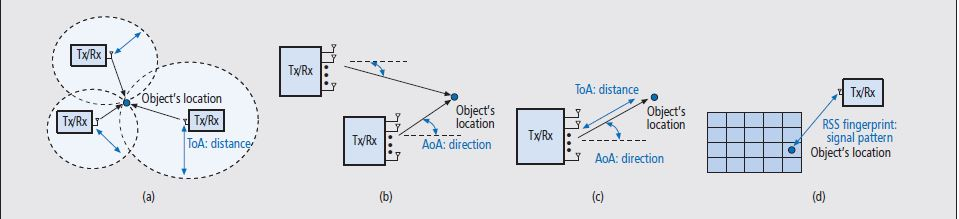
\includegraphics[width=\textwidth]{images/wifi}
    \caption{a) Time of arrival approach; b) angle of arrival approach; c) hybrid ToA/AoA approach; d) received signal strength and
fingerprint approach.}
    \label{fig:wifi1}
\end{figure}
\\
\subsubsection{Time Of Arrival}~\\
ToA is the travel time between the transmitter and the receiver. It can be calculated by the travel time multiplied by the speed of light. In order to calculate the travel time in air, it requires synchronisation between transmitter and receivers. It also requires at least three anchors to construct a 2D plane-domain localization shown in figure \ref{fig:wifi1}a. The positioning is calculated from the signal's bandwidth and the sampling rate. When the signal is sampled in the receiver as depicted in figure \ref{fig:wifi1}, the first sample which is captured is not ToA. If the signal's bandwidth is not wide enough, the measurement of the ToA may reslt in a wide error range of distance.\cite{toaerror}\\
\subsubsection{Angle of Arrival}~\\
AoA is a method that determines the incoming signal direction from the transmitter on the antenna array. Exploiting and detecting the phase difference among the antennas can aid in calculation of the direction of the incoming signal. To determine the position, this method requires two anchors array at different places to obtain the position of the object as shown in figure \ref{fig:wifi1}b. However, it is very hard to obtain the AoA in terms of Line of sight (LOS) due to multi path affection.\cite{aoaerror}\\
\subsubsection{Hybrid ToA/AoA}~\\
With this approach, instead of only using just AoA or ToA and to counter the effects of complicated indoor environment and the limited amount of anchors nearby, both values from AoA and ToA are used to calculate localization. This method results in the number of nearby anchors needed to be reduced. As shown in figure \ref{fig:wifi1}c, it is possible to make use of only one nearby anchor to do localization. Although this approach utilizes both ToA and AoA and leverages on the benefits that each approach brings about, it still suffers from the problem of signal bandwidth as well as the number of antennas. \cite{hybrid}\\
\subsubsection{Received Signal Strength and Fingerprint}~\\
Received signal strength (RSS) and fingerprint is a method that leverages on both the RSS as well as the fingerprints. RSS ratio reflects the information regarding the distance. Transmitters power can be calibrated with a free-space channel model established by the distance measured and the power at each point. This outputs the corase distance for each anchor. Fingerprint is then used in conjunction with RSS because the signal property such as frequency response and signal strength regarding the I/Q channel has its unique fingerprint due to the multi-path effect. A fingerprint database will then store all the signal fingerprint, which can be associated with the anchor to estimate the location. Only one nearby anchor node is required in this approach, as shown in figure \ref{fig:wifi1}. This approach however requires a sit survey to be done in advance and if the indoor environment is dynamic such as a shopping mall with moving crowd, it can affect and degrade the performance of the approach. As the fingerprint database increases exponentially, the calculations required to estimate location increases too. \cite{rss}\\
\subsubsection{Proposed Improvements}~\\
As the conventional approaches have each of their own limitations, the paper discusses an alternate approach which improves on the current existing ToA and AoA implementation.\\
\subsubsection{Super-Resolution ToA and Performance Improvement}~\\
\FloatBarrier
\begin{figure}[h]
    \centering
    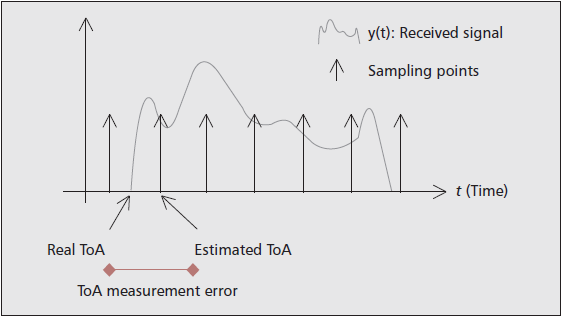
\includegraphics[width=120mm]{images/toa}
    \caption{ToA performance vs transmitter bandwidth}
    \label{fig:toa1}
\end{figure}
ToA's performance is usually decided by the signal bandwidth and sampling rate. If the bandwidth is narrow, the ToA's readings may not be captured accurately. As shown in figure \ref{fig:toa1}, the black arrows denotes the sampling of the received signal while the real ToA signal sit in between two sampling positions. This results in a measurement error. In order to counter this, the method super-resolution estimation is employed. This method is based on the subspace decomposition of the autocorrelation matrix and requires the calculation of an inverse matrix with its eigenvectors. The problem with this is that it requires heavy calculation loading without actually improving the performance.\cite{superreso}\\
\subsubsection{The improvement to ToA}~\\
\FloatBarrier
\begin{figure}[h]
    \centering
    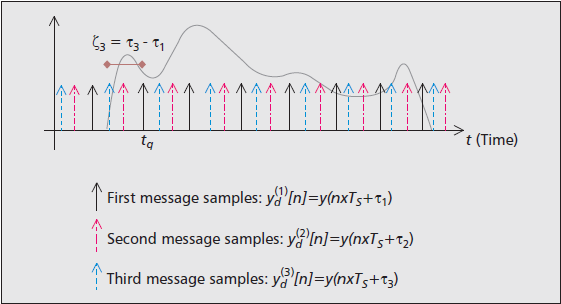
\includegraphics[width=\textwidth]{images/reconstruct}
    \caption{Multiple messages for reconstruction of the received signal}
    \label{fig:recon1}
\end{figure}\\
Even though super-resolution estimation is a state-of-the-art solution to the narrow bandwidth problem faced by ToA, the performance is ultimately decided by the signal bandiwdth. The paper then proposes a alternate method to increase the accuracy of the ToA estimate. By sending multiple of the same predefined messages, it can aid in performing and assisting in estimation, based on the assumption that each incoming message is unlikely to be sampled at the same place and hence, the collection of received messages in linear time invariant (LTI) channels can then reconstruct the received signal at higher resolution. This is shown in figure \ref{fig:recon1}, where the formulas for the first to second and finally the third message sample is shown - yd (i)[n] = y[n × Ts + ti]. The i in the formula is denoted as the ith message after sampling in the receiver. With the ith and jth messages after sampling using yd (i)[n] = y[n × Ts + ti] and yd (j)[n] = y[n × Ts + tj], the time difference between the two messages can be calculated by applying dt = tj – ti. For fast Fourier transform (FFT) size N, the DT can be calculate by applying the time shift property at subcarrier K as \\
\begin{equation*} \delta_{t}=\frac{\angle Y_{d}^{j}[K]-\angle Y_{d}^{i}[K]}{2\pi\frac{K}{NT_{s}}}\ \text{for}\ K\in 0,1,2,\ldots, N-1\tag{1} \end{equation*}\\
 However, if there are no packets received on the receiver due to congestion or heavy collisions, the estimated time cannot be calculated and obtain. The reconstruction of the signal also relies on finding the sample of a message that is the closest to the arrival signal.\cite{improvetoa}\\
\subsubsection{AoA Approaches and Constraint Improvements}~\\
Generally, AoA is measured by using the phase difference of arrival signal among multiple antennas. However, the received signal will suffer from the combinations of multiple rays with different AoA if the incoming messages suffers from multi-path effects. When the ray representing the Line of sight is unclear, the Line of sight AoA information cannot be obtained. Another approach is the joint angle and delay estimation (JADE method)\cite{jade} . However, this method requires a many times larger matrix for calculation. The number of antennas also needs to be larger than the number of multipaths, increasing the complexity of implementation of this approach.\cite{aoaproblems}\\
\subsubsection{The improvement to AoA}~\\
\FloatBarrier
\begin{figure}[h]
    \centering
    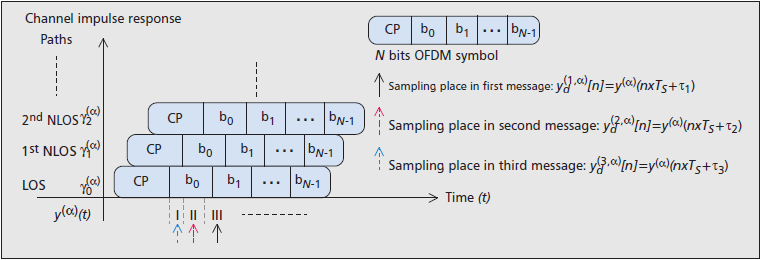
\includegraphics[width=\textwidth]{images/aoa}
    \caption{AoA estimation through channel impulse response.}
    \label{fig:aoa1}
\end{figure}
In order to recover from the effect of multi-path, the paper suggests a novel method to obtain AoA reading from the LOS signal. \texttt{Considering a receiver equipped with NA antennas, the transmitter sends the predefined message x(t) to the ath antenna of a receiver through wireless multipath channel h(a)(t) = g0 (a)d(t) + SLi =1 gi (a)d(t – hi) for a = 1, 2, ..., NA. The received signal y(a)(t) can be described as y(a)(t) = x(t)  h(a)(t). We denoted yd (i,a)[n] as the ith received message after sampling in the ath antenna.} In figure \ref{gif:aoa1}, the received signal is the combination of multiple OFDM symbols with each of their delayed times from the multi-path effect. If the channel state information for each ray can be obtained, the LOS and the AoA can be extracted. For OFDM systems, the channel state information can be obtained through channel estimation techniques from pilot assistances of the ith message hence:\\
\begin{equation*} \hat{h}^{(i, a)}[n]=\text{IFF}\left\{H_{E}(\frac{Y_{d}^{(i, a)}(K)}{X(K)})\right\}\tag{2} \end{equation*}\\
From the equation, N is the Fast Fourier Transformation size, X(K) is the pilot in the K sub-frequency domain and H is the channel estimation approach for estimating the whole frequency response through pilot interpolation.\\
However, traditional approaches requires a certain number of antennas to overcome the multi-path effect. As the multi-path effect grows, the number of required antennas also increases to estimate the AoA.\cite{improveaoa}\\
\subsubsection{System Design}~\\
In the paper, the proposed design consists of Wi-Fi Access Point (AP) where each AP is equipped with N numbers of antenna and the mobile device is equipped with a single antenna. The Round Trip Time (RTT) is then calculated to obtain distance without time synchronization between transmitter and receiver. Transmitter will send a burst of messages while recording the timestamp of the first message. Receiver will used the proposed ToA approach to measure the arrival timestamp of the first message and allocate the response time started.
\begin{equation*} \text{RTT}=(t_{R}-t_{S})\text{modulo}\ T_{U} \end{equation*}
\cite{design}\\
\subsubsection{Localization Procedure}~\\
Once the angle and distance has been calculated, the localization procedure is visualized as follows:
\begin{itemize}
\item
\textbf{User device:} Requests positioning service of the AP
\item
\textbf{WiFi AP:} Starts sending request for RTT measuring. Once the request is granted, a bursts of message is sent by the AP and the timestamp of first message is recorded.
\item
\textbf{User device:} Device will measure arrival time and responds with burst of messages for RTT measurement. Device will also reconstruct the received signal by re-ordering the M messags with relative time difference. User device also chooses arbitrary i for the sending time i × N × TS to send the burst M messages.
\item
\textbf{Wifi AP:} Measures the RTT and AoA in terms of the user device. The distance is the RTT multiplied by light speed divided by 2, which the RTT is the time difference between sending time and receiving time. AoA is measured by using the message nearest to the ToA to estimate channel state information. WiFi AP then returns its own reference location, distance and direction back to user device.
\item
\textbf{User device:} Uses AoA/ToA to locate its own position and sends request to other AP.
\end{itemize}\cite{localprocedure}\\
\subsubsection{Performance Analysis}~\\
Based on the proposed approach, it is stated that the proposed solution can improve the ToA resolution as comparing to implementing the state-of-the-art super-resolution method under limited signal bandwidth without the need for the heavy calculation loading. With the sending of multiple message assistance, it is concluded that the number of antennas required can be reduced. With more than one AP in an indoor environment, the accuracy of the localization can be further improved by joint positioning. The proposed approach boast superior performance improvements without changing any hardware settings.\cite{conclusion}\\
\subsubsection{Limitations of Wi-Fi based System}~\\
Even with the positive results and analysis from the study, there are still several challenges in implementing an indoor positioning system using Wi-Fi technology. Generally, as nearby anchors are heavily relied on in a Wi-Fi-based approach, the cost of deploying such anchors are high. Similarly, it is also expensive to develop such localization devices to identify and communicate with the anchors.\\
In an indoor environment, due to the limited space available, there is a constraint to number of nearby anchors that can be properly deployed, affecting the accuracy of the system. Wi-Fi-based positioning systems also suffer from signal inteferences due to structures such as walls, objects or human beings and leads to multi-path effects.\\
The paper also listed several limitations that the different conventional approaches has brought about - mainly the signal bandwidth problem that may lead to a wide range of error if it is not wide enough, the Line of sight (LOS) being difficult to obtain due to multi-path effects and the potential exponential increase of the calculations on an ever-growing fingerprint database.\\
Hence, Wi-Fi alone is not the best solution for tackling a problem like an Indoor Positioning System.\\

\subsection{Bluetooth}
The other approach in an RF-based localization system is the use of Bluetooth. With many Bluetooth Low Energy devices being widely deployed, this form of localization has now become a much more practical solution to the existing indoor localization system's apparent issues. A study conducted proposes two different novel approach through Low-Precision Indoor Localization (LIL) as well as High-Precision Indoor Localization (HIL) using the RSSI data collected.\cite{blerssi}\\
This approach has been taken due to the issues with GPS not working efficiently enough in an indoor environment as the line of sight is required in the GPS approach and when the LOS is not obtainable, the GPS approach cease to function. \cite{gpsproblem}\\
In this study, the proposed methods of generates the region of the object where it is to be found while making use of the RSSI measurement.
\subsubsection{Low-Precision Indoor Localization}~\\
\begin{figure}[h]
    \centering
    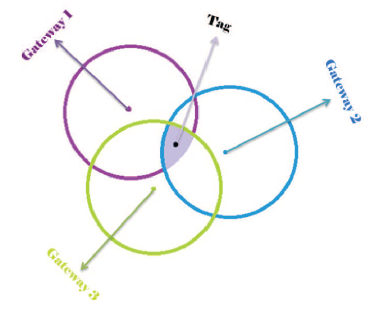
\includegraphics[width=50mm]{images/lil}
    \caption{Tag within the Transmission Range of Multiple Gateways}
    \label{fig:lil1}
\end{figure}\\
LIL was proposed as there is fluctuation in the readings from the RSSI, and with LIL< it achieves comrpomised localization precision using different power levels.\cite{lil}. The problem identified by the authors of the study was that whether the gateway receives the signals from the RSSI. As each transmission power of the tag has a maximum range limit, any value beyond this limit will result in the gateway being unable to receive the RSSI signals. As depicted in figure \ref{fig:lil1}, each circle denotes a gateway while the radius of the circle represents the transmission rate limit. At any point in time one of the gateway receives the RSSI signal, the circle of that gateway will be highlighted. If there are multiple gateways receiving the same RSSI signals, the overlapping region of the circles will be highlighted. With that, it can be assumed that the highlighted region is the most possible locaiton of the tag and with this data, the team in the study developed a matrix-based determination method returning the coordinates of the overlapping region.\cite{matrix}\\
\begin{figure}[h]
    \centering
    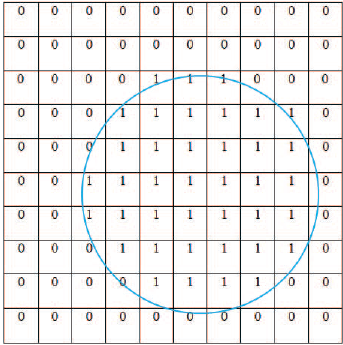
\includegraphics[width=50mm]{images/matrix}
    \caption{An example of 10x10 Matrix-Based Determination}
    \label{fig:matrix1}
\end{figure}\\
The matrix-based determination technique helps to identify within the matrix cells the coverage of a gateway, as shown in figure \ref{fig:matrix1}, where the values of the matrix cells within the circle are 1 and the cells outside are 0.\\
Together with the Matrix-based determination, the team also used logic AND operation on all the experimental matrixes to deduce the final location region. However, LIL approach is only able to produce a rough estimation of the location range. If the transmission range limit is very large for high power levels, the location of the tag will be in a larger region. This only leads to inaccuracy in denoting the location.\cite{problemlil}\\
\subsubsection{High-Precision Indoor Localization}~\\
In order to counter the rough location provided by LIL, the team has developed a HIL approach based on the LIL method - by splitting up different power ranges into smaller bands so as to enhance the precisioning. In order to kick start the HIL scheme, a RSSI data-training phase is required, where the team collects a bunch of RSSI samples every meter and applies the 68-95-99.7 Rule \cite{filterrule} to filter out non-normal sample data. \cite{hil}\\
The team made use of the Bluegiga USB dongle as a gateway and a RadBeacon tag - a fully standalone Bluetooth proximity beacon as the tag and proceeded to conduct the experiment in a similar fashion like the LIL approach. The procedure is as follows:
\begin{itemize}
\item
Generating tag's random location and calculating distance to all gateways deployed.
\item
Use a binary search algorithm to look for shortest distance to every gateway in the training data generated.
\item
Choose a random RSSI measurement that corresponds to the shortest distance as the simulated RSSI for that particular gateway. If the shortest distance is covered by both high and low power range, then there will be two simulated measurements chosen.
\item
The above steps are then repeated for the other gateways to generate the simulated RSSI measurements.
\item
With all the calculated simulated RSSI measurements, apply the data training to find the corresponding distance band and apply the Matrix-based determination to locate the band.
\item
Finally, perform the logic AND operation on all the experimental matrixes to find the ultimate band. If the tag is outside the ultimate band, it will revert to applying LIL.
\end{itemize}
\pagebreak
\subsubsection{Results}~\\
\begin{figure}[h]
\centering
\subfloat[Matrix resolution at 0.05m]{{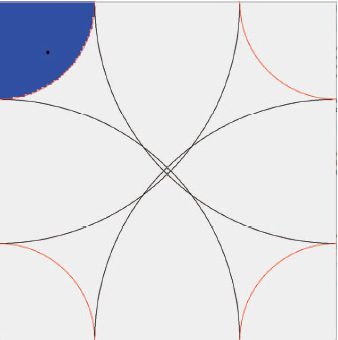
\includegraphics[width=5cm]{images/matrixreso}}}
\qquad
\subfloat[Matrix resolution at 0.5m]{{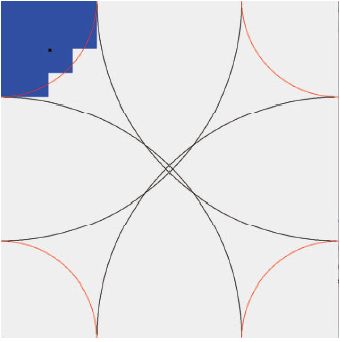
\includegraphics[width=5cm]{images/matrixresosmaller}}}
\caption{Comparison of different Matrix Resolution}
\label{fig:matrixreso1}
\end{figure}\\
\begin{figure}[h]
\centering
\subfloat[Low-Precision Indoor Localization Results]{{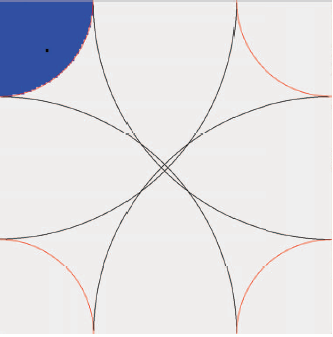
\includegraphics[width=5cm]{images/lilresult}}}
\qquad
\subfloat[High-Precision Indoor Localization Results]{{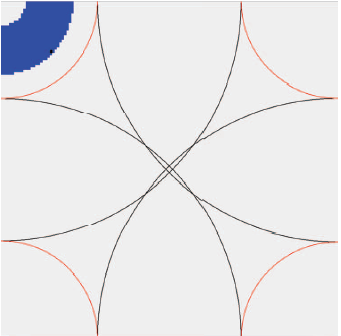
\includegraphics[width=5cm]{images/hilresult}}}
\caption{Comparison of HIL v.s. LIL}
\label{fig:lilhil1}
\end{figure}\\
Firstly, comparing different Matrix Resolution as denoted at figure \ref{fig:matrixreso1}, it can be said that with a smaller Matrix Resolution, it is more accurate, however at a higher computational costs.\\
Comparing both the results of LIL and HIL denoted at figure \ref{fig:lilhil1}, it can be seen that the ulitmate band calculated using the HIL approach is significantly smaller and more accurate than the band computed by the LIL approach.\\
\subsubsection{Problems with Bluetooth-based Systems}~\\
Even though the HIL approach discussed in the paper has shown significant improvement in terms of accuracy in the localization as compared to the LIL approach, there are still several issues with a Bluetooth-based Indoor Positioning System (IPS). Because a Blueooth-based system rely on the RSSI measurements, such measurements are also susceptible to multi-path fading attenuation and interference that can cause the RSSI measurements to fluctuate in an indoor environment, leading to inaccurate positioning results.\\
Similarly, there is a need to install multiple BLE beacons within an indoor environment to faciliate the estimation of the location with a Bluetooth-based IPS. This will result in an increase in the overall cost. The system will suffer from errors like positioning misplacement to nearby positions and position losses where the application cannot determine the position due to lack of signal coverage. -- add in the word doc link., maybe add in another paper.

\section{Sensor-based Systems}
Another approach commonly taken for the implementation in an Indoor Positioning System is the sensor-based systems, otherwise known as Sensor Fusion. This approach combines the reading from sensors like accelerometer, gyroscope and other sensors to do localization estimation. One such study proposed a position estimation algorithm with the data from a smartphone's accelerometer, gyroscope and magnetometer. The fusion of accelerometer and gyroscope values produces the pitch and roll vlaues, where the pitch value is used for step detection. Step length is then calculating by using the pitching amplitude. To determine the heading of the smartphone, the fusion of magnetometer and gyroscope values are used. The distance is then finally estimated using the heading and the step length.\cite{imu}\\
\subsection{Smartphone Coordinate System}
\begin{figure}[h]
    \centering
    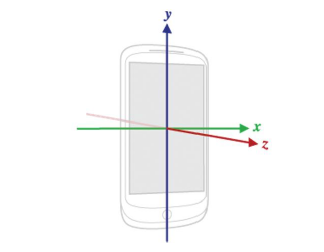
\includegraphics[width=70mm]{images/smartphone}
    \caption{Smartphone coordinate system (relative to a device)}
    \label{fig:smartphone1}
\end{figure}\\
In the study, the team proposed a sensor fusion technique using only embedded sensors that can be found within the smartphone to calculate pitch and roll, pitch-based step detection, heading estimation as well as positioning estimation.\\
A general smartphone's sensor consists of a 3-axis coordinate system to express data values. The coordinate system of the smartphone is relative to the screen of the device in its default orientation as shown in figure \ref{fig:smartphone1}. The X-axis is horizontal and points to the right, the Y-axis is vertical and points upwards while the Z-axis points out from face of the screen. These axes do not swap when the device orientation change, meaning that the coordinate system never changes as the device moves. This can be defined in a rotation matrix as shown
\begin{equation*} \boldsymbol {R} = \left [{ {\begin{array}{*{20}{c}} {E_{x}}&\quad {E_{y}}&\quad {E_{z}}\\ {N_{x}}&\quad {N_{y}}&\quad {N_{z}}\\ {G_{x}}&\quad {G_{y}}&\quad {G_{z}} \end{array}} }\right]\tag{1}\end{equation*}. X, Y and Z are the axes relative to the smartphone and E is a unit vector pointing to the East while N is a unit vector pointing to the North. G on the other hand is a unit vector pointing away from center of the earth, also known as the gravity vector.\\
The Euler angle is also discussed in this paper where the Euler angles Φ,θ and ψ are expressed as
\begin{align*} \textrm {azimuth}=&\psi = \textrm {rotation about}~ {\boldsymbol {G}.} \\ \textrm {pitch}=&\theta = \textrm {rotation about}~ {\boldsymbol {E}.} \\ \textrm {roll}=&\Phi = \textrm {rotation about}~ {\boldsymbol {N}.}\end{align*} \cite{euler}.\\
As a smartphone device moves, there is a tilting effect that needs to be removed. The paper discusses their way of removing such tilting effects by transforming the original acceleration data from smartphone coordinates to earth coordinate system, expressed as follows
\begin{align*} {\boldsymbol {R}_\psi }=&\left [{ {\begin{array}{*{20}{c}} {\cos \psi }&\quad {\sin \psi }&\quad 0\\ { - \sin \psi }&\quad {\cos \psi }&\quad 0\\ 0&\quad 0&\quad 1 \end{array}} }\right] \tag{2}\\ {\boldsymbol {R}_\theta }=&\left [{ {\begin{array}{*{20}{c}} 1&\quad 0&\quad 0\\ 0&\quad {\cos \theta }&\quad {\sin \theta }\\ 0&\quad { - \sin \theta }&\quad {\cos \theta } \end{array}} }\right] \tag{3}\\ {\boldsymbol {R}_\phi }=&\left [{ {\begin{array}{*{20}{c}} {\cos \phi }&\quad 0&\quad {\sin \phi }\\ 0&\quad 1&\quad 0\\ { - \sin \phi }&\quad 0&\quad {\cos \phi } \end{array}} }\right]\tag{4}\end{align*}\cite{tilting}\\ and the transformation of the acceleration data to earth coordinate can be represented as
\begin{equation*} \left [{ {\begin{array}{*{20}{c}} {A_{x}}\\ {A_{y}}\\ {A_{z}} \end{array}} }\right] = {\boldsymbol {R}_{\left ({{\psi, \theta, \phi } }\right)}}{\left [{ {\begin{array}{*{20}{c}} {a_{x}}&\quad {a_{y}}&\quad {a_{z}} \end{array}} }\right]^{T}}\tag{5}\end{equation*}
\\
and then removing the effect of gravity can be represented as
\begin{equation*} {\boldsymbol {A}_{\textrm {linear}}} = \left [{ {\begin{array}{*{20}{c}} {A_{x}}\\ {A_{y}}\\ {A_{z}} \end{array}} }\right] - g{\left [{ {\begin{array}{*{20}{c}} 0&\quad 0&\quad 1 \end{array}} }\right]^{T}} \tag{6}\end{equation*}which is the calculation for linear acceleration and g is 9.8, which is the gravitational acceleration.
\subsection{The proposed algorithm for Indoor Localization}
\begin{figure}[h]
    \centering
    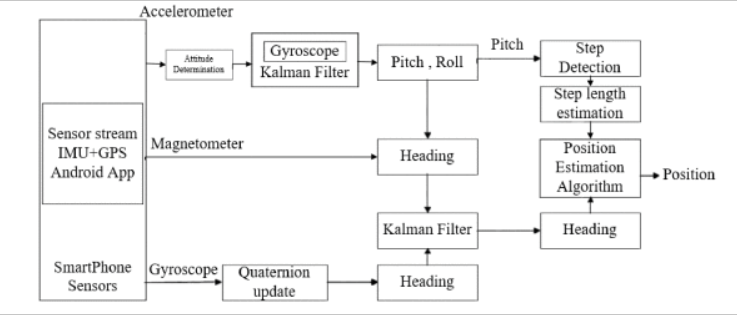
\includegraphics[width=70mm]{images/estalgo}
    \caption{Smartphone-based position estimation}
    \label{fig:estalgo1}
\end{figure}\\
The study combines the sensor readings from accelerometer, magnetometer and gyroscope shown in figure \ref{fig:estalgo1}. Data was collected by the team using the sensor stream inertial measurement unit and a global positioning android system application.\cite{datacollect}. Firstly, the pitch and roll was calculated with the pitch being utilised for step detection which was then used for step length calculation. Heading was determined using the gyroscope and magnetometer sensor readings and with the step length and heading, the positoning was estimated.
\subsubsection{Pitch and Roll Estimation}~\\
Sensor fusion is a technique utilised that combines multiple sensor values to calculate a certain value. In this case, the sensor readings from the embedded accelerometer and gyroscope from a smartphone is used to calculate the pitch and roll. The reasoning for doing a fusion with accelerometer and gyroscope is so that both the benefits of the individual sensors can be brought together to achieve a better overall performance, with accelerometer good for a longer time span and the gyroscope being good in a short time span.\\
In order to calculate the pitch and roll, the angle is calculated, as denoted by
\begin{align*} \textrm {Pitch angle}(\theta)=&{\sin ^{ - 1}}\left ({{\frac {a_{y}}{g}} }\right) \tag{7}\\ \textrm {Roll angle}(\phi)=&{\tan ^{ - 1}}\left ({{\frac {a_{x}}{a_{z}}} }\right)\tag{8}\end{align*}\\
\begin{figure}[h]
    \centering
    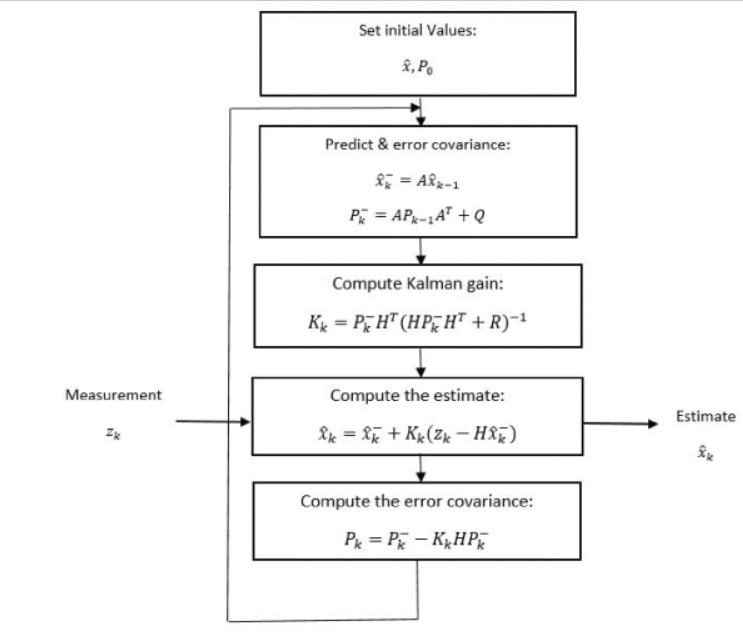
\includegraphics[width=70mm]{images/kalman}
    \caption{Kalman Filter Algorithm}
    \label{fig:kalman1}
\end{figure}\cite{kalmanalgo}\\
In order to reduce the accumulated errors from the numerical integration, the calculated values is pass through a Kalman filter\cite{kalmanfilter} to produce better results which is visualised in figure \ref{fig:kalman1}. The gyroscope quaternion values are used as state variables, denoted by 
\begin{equation*} \boldsymbol {x} = \big[{\begin{array}{*{20}{c}} {q_{0}}&\quad {q_{1}}&\quad {q_{2}}&\quad {q_{3}}\big] \end{array}^{T}}\tag{9}\end{equation*}\\
The three-axis gyroscope data in the device coordinate systems are (ωx,ωy,ωz) and the quaternion-based state update above is given by
\begin{equation*} \dot {\boldsymbol {q}} = \frac {1}{2}\left [{ {\begin{array}{*{20}{c}} 0&\quad { - {\omega _{x}}}&\quad { - {\omega _{y}}}&\quad { - {\omega _{z}}}\\ {\omega _{x}}&\quad 0&\quad {\omega _{z}}&\quad { - {\omega _{y}}}\\ {\omega _{y}}&\quad { - {\omega _{z}}}&\quad 0&\quad {\omega _{x}}\\ {\omega _{z}}&\quad {\omega _{y}}&\quad { - {\omega _{x}}}&\quad 0 \end{array}} }\right]\left [{ \begin{array}{l} {q_{0}}\\ {q_{1}}\\ {q_{2}}\\ {q_{3}} \end{array} }\right]\tag{10}\end{equation*}\\
The system model matrix is then defined as
\begin{equation*} \boldsymbol {A} = \frac {1}{2}\left [{ {\begin{array}{*{20}{c}} 0&\quad { - {\omega _{x}}}&\quad { - {\omega _{y}}}&\quad { - {\omega _{z}}}\\ {\omega _{x}}&\quad 0&\quad {\omega _{z}}&\quad { - {\omega _{y}}}\\ {\omega _{y}}&\quad { - {\omega _{z}}}&\quad 0&\quad {\omega _{x}}\\ {\omega _{z}}&\quad {\omega _{y}}&\quad { - {\omega _{x}}}&\quad 0 \end{array}} }\right]\tag{11}\end{equation*}\\
As the state variable is defined by the gyroscope quaternion values, it is necessary to convert those data to quaternion values, which is visualized as such
\begin{align*} \left [{ \begin{array}{l} {q_{0}}\\ {q_{1}}\\ {q_{2}}\\ {q_{3}} \end{array} }\right] = \left [{ \begin{array}{*{20}{c}} {\cos \frac {\phi }{2}\cos \frac {\theta }{2}\cos \frac {\psi }{2} + \sin \frac {\phi }{2}\sin \frac {\theta }{2}\sin \frac {\psi }{2}}\\[0.4pc] {\sin \frac {\phi }{2}\cos \frac {\theta }{2}\cos \frac {\psi }{2} - \cos \frac {\phi }{2}\sin \frac {\theta }{2}\sin \frac {\psi }{2}}\\[0.4pc] {\cos \frac {\phi }{2}\sin \frac {\theta }{2}\cos \frac {\psi }{2} + \sin \frac {\phi }{2}\cos \frac {\theta }{2}\sin \frac {\psi }{2}}\\[0.4pc] {\cos \frac {\phi }{2}\cos \frac {\theta }{2}\sin \frac {\psi }{2} - \sin \frac {\phi }{2}\sin \frac {\theta }{2}\sin \frac {\psi }{2}} \end{array}}\right]\quad \tag{12}\end{align*}
\\
The H matrix in figure \ref{fig:kalman1} is given by
\begin{equation*} \boldsymbol {H} = \left [{ {\begin{array}{*{20}c} 1 &\quad 0 &\quad 0 &\quad 0 \\ 0 &\quad 1 &\quad 0 &\quad 0 \\ 0 &\quad 0 &\quad 1 &\quad 0 \\ 0 &\quad 0 &\quad 0 &\quad 1 \\ \end{array}} }\right]\tag{13}\end{equation*} and the noise covariance matrices Q and R are expressed as
\begin{align*} \boldsymbol {R}=&\left [{ {\begin{array}{*{20}{c}} {0.0001}&\quad 0&\quad 0&\quad 0\\ 0&\quad {0.0001}&\quad 0&\quad 0\\ 0&\quad 0&\quad {0.0001}&\quad 0\\ 0&\quad 0&\quad 0&\quad {0.0001} \end{array}} }\right] \tag{14}\\ \boldsymbol {Q}=&\left [{ {\begin{array}{*{20}{c}} {0.001}&\quad 0&\quad 0&\quad 0\\ 0&\quad {0.001}&\quad 0&\quad 0\\ 0&\quad 0&\quad {0.001}&\quad 0\\ 0&\quad 0&\quad 0&\quad {0.001} \end{array}} }\right]\tag{15}\end{align*}\\

The initial value for the state variable is given as the following form
\begin{equation*} \tilde {\boldsymbol {x}}= \big[\begin{array}{*{20}{c}} 1&\quad 0&\quad 0&\quad {0}\big]^{T} \end{array}\tag{16}\end{equation*} while the error covariance matrix is represented as
\begin{equation*} \boldsymbol {P}_{0} = \left [{ {\begin{array}{*{20}c} 1 &\quad 0 &\quad 0 &\quad 0 \\ 0 &\quad 1 &\quad 0 &\quad 0 \\ 0 &\quad 0 &\quad 1 &\quad 0 \\ 0 &\quad 0 &\quad 0 &\quad 1 \\ \end{array}} }\right]\tag{17}\end{equation*}\cite{kalmanfilter}\\

\subsubsection{Step Detection}~\\
\begin{figure}[h]
    \centering
    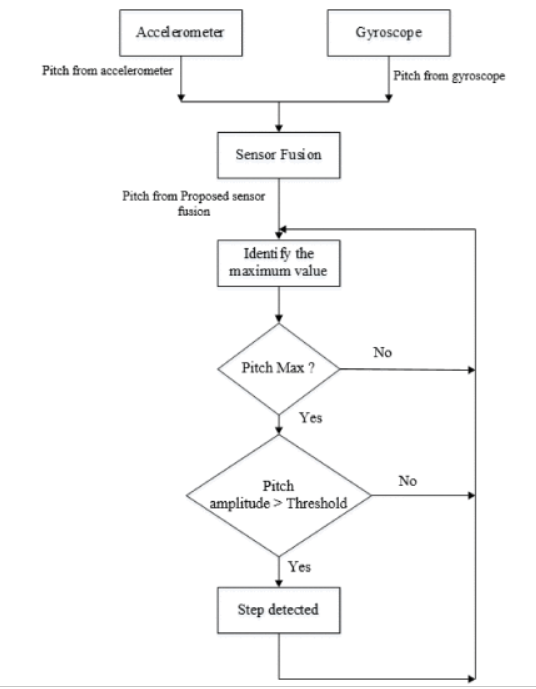
\includegraphics[width=70mm]{images/pitch}
    \caption{Pitch based step detector}
    \label{fig:pitch1}
\end{figure}\\
With the pitch and roll values being calculated using sensor fusion with the accelerometer and gyroscope data, the pitch value can then be used to detect when a step is taken. The idea of a pitch-based step detection is explain in \cite{pitchbased}. A step is detect when the maximum pitch value occurs. The proposed pitch based step detector is shown in figure \ref{fig:pitch1}. There is a maxima and minima where maxima is a maximum peak exceed the upper threshold while minima is the minumum peak lower than the lower threshold. In order to avoid having false steps analysed, it must exceed the upper limit threshold value.
\subsubsection{Step Length Estimation}~\\
\begin{figure}[h]
    \centering
    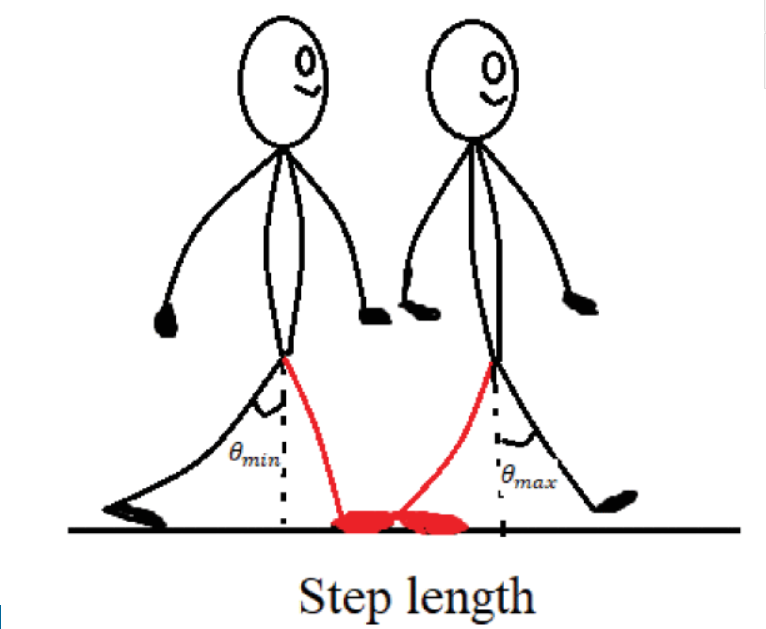
\includegraphics[width=70mm]{images/steplength}
    \caption{Humans' legs during occurence of a step}
    \label{fig:step1}
\end{figure}\\
figure \ref{fig:step1} shows how a step occurs in a human walking. In order to estimate the step length, it is estimated through a first-order linear regression model on the pitch amplitude  (Δθ ) and is denoted as 
\begin{equation*} SL = a \times \Delta \theta + b\tag{18}\end{equation*}
where Δθ is the difference between highest positive peak (θmax ) and lowest negative peak (θmin ), in degrees. The constants a and b are the personalized parameters fitting each regression line.\cite{steplengthestimate}.

\subsubsection{Heading Estimation}~\\
Another important piece of data required for the positioning estimation is the heading. Heading is the estimate of the direction of the pedestrian. To calculate heading, the readings of the gyroscope and magnetometer sensors are used. Similarly, sensor fusion tehcnique is applied in order to reduce the errors during a long time span. The relation between magnetic strength in the device (hx, hy, hz) and global (Hx, Hy, Hz) coordinate system is expressed as
\begin{align*} \left [{ \begin{array}{l} {H_{x}}\\ {H_{y}}\\ {H_{z}} \end{array} }\right] = \left [{ {\begin{array}{*{20}{c}} {\cos \phi }&\quad {\sin \phi \sin \theta }&\quad { - \sin \phi \cos \theta }\\ 0&\quad {\cos \theta }&\quad {\sin \theta }\\ {\sin \phi }&\quad { - \sin \theta \cos \phi }&\quad {\cos \phi \cos \theta } \end{array}} }\right]\left [{ \begin{array}{l} {h_{x}}\\ {h_{y}}\\ {h_{z}} \end{array} }\right]\!\!\!\!\! \\\tag{19}\end{align*}\\
Heading γ is then given by\begin{equation*} \gamma = {\tan ^{ - 1}}\left ({{\frac {H_{y}}{H_{x}}} }\right) \tag{20}\end{equation*}\\
To compute the Euler angles \cite{eulerangle}, the paper stated let ωx represent the body-frame x -axis gyro output, ωy represent the body-frame y -axis gyro output, and ωz represent the body-frame z -axis output and the angles are computed as
\begin{align*} \left [{ {\begin{array}{*{21}{c}} {\omega _{x} + {\omega _{y}}\sin (\phi)\tan (\theta) + {\omega _{z}}\cos (\phi)\tan (\theta)}\\ {\omega _{y}\cos (\phi) - {\omega _{z}}\sin (\phi)}\\ {\omega _{y}\sin (\phi)/\cos (\theta) + {\omega _{z}}\cos (\phi)/\cos (\theta)} \end{array}} }\right] = \left [{ {\begin{array}{*{22}{c}} {\mathop \phi \limits ^{.} }\\ {\mathop \theta \limits ^{.} }\\ {\mathop \psi \limits ^{.} } \end{array}} }\right] \\\tag{21}\end{align*}\\
Using the quaternion update values, the gyroscopic heading is obtaied by
\begin{equation*} \textrm {Heading}{_{\textrm {gyro}}} = \arctan \left [{ {\frac {{2({q_{0}}{q_{3}} + {q_{1}}{q_{2}})}}{1 - 2(q_{2}^{2} + q_{3}^{2})}} }\right]\tag{22}\end{equation*}\\
The position estimation algorithm make use of the results from the Heading γ (20) and gyroscopic heading (22) for sensor fusion.\\
The heading direction is then calculated as 
\begin{equation*} {S_{t}} = A{S_{t - 1}} + B\gamma +w\tag{23}\end{equation*}
where A and B are identity matrices and w denotes the Gaussian noise of the system with zero mean and variance ϕ . The observation of the system comes from the gyroscope sensor output. The observation function can be expressed as
\begin{equation*} {O_{t}} = C{S_{t }}+ r\tag{24}\end{equation*} where C = [1 0] and r denotes the Gaussian noise of the magnetometer output with zero mean and variance.\\
Kalman filter is then applied to solve the problem in the predicting
\begin{align*} {S_{t}}=&A{S_{t - 1}} + B\gamma \tag{27}\\ {P_{t}}=&A{P_{t - 1}}{A^{T}} + \phi\tag{28}\end{align*}\\
and the updating
\begin{align*}{K_{t}}=&{P_{t}}{C^{T}}{(C{P_{t}}{C^{T}} + \varphi)^{ - 1}}\tag{29}\\ {S_{t}}=&{S_{t - 1}} + {K_{t}}({O_{t}} - C{S_{t - 1}})\tag{30}\\ {P_{t}}=&{P_{t}} - KC{P_{t}}\tag{31}\end{align*}

\subsubsection{Position Estimation}~\\
Position estimation is finally done making use of the step length and heading information. From a previously known position together with the step length and heading from a step interval\cite{lilkovi}, the current position of the pedestrian is then calculated. Assumption of the initial position of the pedestrian is zero, expressing the position as \begin{align*} X_{t}=&X_{t - 1} + SL \times \cos (HD) \tag{32}\\ Y_{t}=&Y_{t - 1} + SL \times \sin (HD) \tag{33}\end{align*}
where Xt , Yt are the position values and Xt−1 , Yt−1 are the initial position values. To determine the absolute position of the pedestrian, QR code, RFID, UWB, and computer vision navigation methods are used.\cite{positionestimate}\\

\subsection{Conclusion}
With the proposed method from the study, it has shown a higher positioning accuracy as compared to the conventional approaches due to the use of sensor fusion techniques to help reduce accumulated errors as well as the use of complementary features of magnetometer and gyroscope which aid in addressing the existing errors in Pedestrian Dead Reckoning localization. However, even with the sensor fusion technique and the use of filters and complementary features, the proposed solution still suffers from errors. The rectangular motion experiment shows a maximum of 2.6m error when compared to reference path. In the straight line motion, it reflected a maximum of 0.94m error. In the circular motion, the algorithm reflected a maximum of 1.2m error. This infers that the accumulated drift error still occurs within the algorithm.

\section{Quick Response Code}
A Quick Response (QR) Code is a type of matrix barcode, a machine readable optical label containing information about the attached item. It may also contain data for a locator, identifier or a tracker that points to a website or an application. \cite{qrwiki}. With the amount and variety of information that a QR code can store, a study was conducted to determine if QR Code could be used as landmarks for an indoor positioning system.

\subsection{System Design}
In the paper, the proposed solution for using QR Code as a landmark was to make use of a Kinect v2 sensor.\cite{qrcodelm} A Kinect v2 sensor has a high definition RGB camera and a depth sensor. The camera can capture high-definition image and video captured can be displayed on the screen in the same resolution. The RGB camera and the depth sensor will capture the QR Code and decode it to calculate the distance between the code and the sensor.\\
In order to process the image of the QR code being captured, an image processing library is required. One such library used in this study was OpenCV.\cite{openvc}. OpenCV is used to scan the contours within the image and highlight the QR code to indicate if QR Code is successfully captured.\cite{opencvusage} To read the QR code, there are multiple libraries to ulitize. One such library used in this study was Zbar.\cite{zbar} ZBar library is applied to decode the QR codes that is captured in the image.

\subsection{Algorithm and Methodology}
To calculate the exact position of the sensor, trilateration-based positioning was used to do that. The kinect sensor will collect the depth data between the sensor to the QR Code and using the ZBar library to decode the QR Code to retrieve the coordinates encoded. To obtain the 3D position of the sensor, at least 3 QR codes needs to be captured and analysed.\cite{3d}.

The values encoded in the QR code can be defined as (xi,yi,zi), where i=1,2,3 are the exact positions of the QR codes and the distance between the kinect sensor and the QR code can be represented as  di, where i=1,2,3. The whole equation can be shown as
\begin{align*} \sqrt{(x-x_{1})^{2}+(y-y_{1})^{2}+(z-z_{1})^{2}} &= d_{1} \\ \sqrt{(x-x_{2})^{2}+(y-y_{2})^{2}+(z-z_{2})^{2}} &= d_{2} \\ \sqrt{(x-x_{3})^{2}+(y-y_{3})^{2}+(z-z_{3})^{2}} &= d_{3} \end{align*}
With this equation, the exact position of the Kinect sensor can be determine. In the paper, they applied the Newton-Raphson method to calculate the Kinect sensor's position.

\subsection{Conclusion}
Using the Kinect v2 sensor together with OpenCV and ZBar library, the team came to a conclusion that QR code-based landmarks is a feasible option to assist other forms of applications such as robot or user in terms of navigation in an indoor environment. However, it was realised that there were still errors or inaccuracy from the proposed solution as the measuring angle of Kinect depth sensor affected the accuracy of the data and the closer it is to the central region of the sensor, the more accurate the data collected. \cite{qrconclusion}

\section{Hybrid Positioning approaches}
There are many different technologies being implemented for indoor localization, however each technology has their own advantages and disadvantages. In order to overcome the limitations of the individual technologies, hybrid localization approaches can be implemented. \cite[p.~114]{plie}\cite[p.~39-50]{wireless}. 



%==================================================================================================================================
\chapter{Background}
Many different approaches has been applied in the aspect of Indoor navigation. With the increased amount of WiFi access points and Bluetooth low energy beacons emerging in buildings such as shopping malls etc, many applications are making use of that infrastructure to construct a reliable indoor navigation system. However, such systems are susceptible to error due to multi path effect faced, as well as stability of the signals coming from the devices can be affected by the indoor structures. Also, in order to use this approach in new buildings, each building must be equipped with additional infrastructure in order to support this implementation, which leads to additional costs.\\

Smartphones are also growing at an incredible rate, where each smartphone can perform advanced tasks due to the fast advancing rate of smartphone technology. Sensors embedded within the smartphone can be utilised to capture various data and be applied in many fields, indoor positioning being one of it. As this approach does not require any additional installation of infrastructures such as Access Points or beacons, it is a relatively popular approach. However, this approach often leads to inaccuracy because the sensors in the smartphone suffers from drift error.\\

In order to improve on the existing smartphone sensor-based approach, Quick response code can be introduced into a sensor-based system, creating a hybrid approach. The QR Code can help to realign the smartphone’s position that is being calculated from the sensors after the drift error accumulates. This ensures that even if the position is incorrect due to the drift error, the QR Code can help calibrate and reset the position of the smartphone.\\

This hybrid method is proposed as opposed to using WiFI AP or BLE is because of cost. Cost plays an important factor in determining the approach selected. The cost of a single wireless access point can range from thisval to thisval (check) while a BLE can cost from thisval to thisval. Comparing these prices to a smartphone which is a necessity in most of the people’s lives today, it is relatively more expensive to install AP or BLE. In an indoor environment, the whole building would also require more than a single AP or BLE. Quick Response code can also be generated online without a cost and the information encoded in the QR code is flexible, which can be determined by the developer themselves, hence the hybrid approach of smartphone embedded sensor and QR code is chosen.\\


%==================================================================================================================================
\chapter{Analysis/Requirements}
What is the problem that you want to solve, and how did you arrive at it?
\section{Guidance}
Make it clear how you derived the constrained form of your problem via a clear and logical process. 

%==================================================================================================================================
\chapter{Design}
In the discussed implementation, an android smartphone application is developed, making use of the smartphone's embedded sensor together with the smartphone camera to detect the QR Code which will then bring the smartphone's position back to the correct position.
\section{Basic Architecture}
\begin{figure}[h]
    \centering
    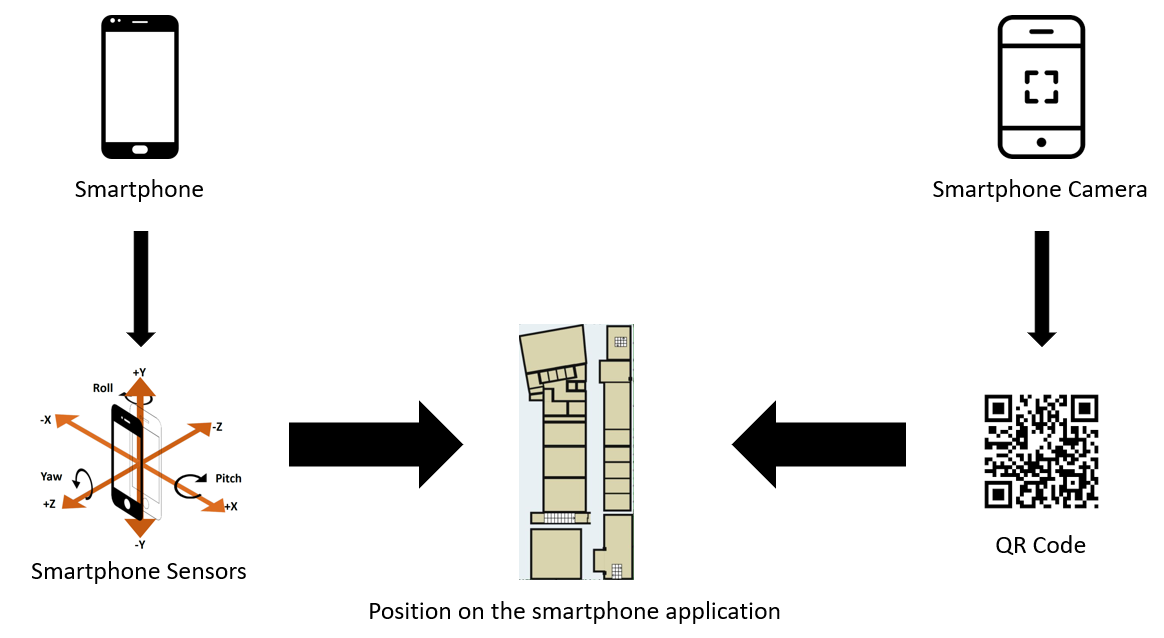
\includegraphics[width=70mm]{images/architect}
    \caption{Smartphone positioning application architecture}
    \label{fig:architecture1}
\end{figure}\\

The above figure \ref{fig:architecture1} shows a simple diagram of how the whole application works. The smartphone provides the sensors such as accelerometer, gyroscope, magnetometer and step detector which then provides the data that calculates the orientatiion of the smartphone.\\
The smartphone camera is then used to detect QR codes which helps to bring the smartphone position back to the correct position when it drifts away.
The usage of both the smartphone's sensors and the scanning of the QR code will results in a reliable indoor positioning system.

%==================================================================================================================================
\chapter{Implementation}
For the smartphone application, the tools used are Android Studio for the development of the positioning application, as well as ZXing Library for the QR Code decoding aspect. The application is tested on a Huawei P20 Pro smartphone.
What did you do to implement this idea, and what technical achievements did you make?
\section{Guidance}
You can't talk about everything. Cover the high level first, then cover important, relevant or impressive details.



\section{General points}

These points apply to the whole dissertation, not just this chapter.



\subsection{Figures}
\emph{Always} refer to figures included, like figure \ref{fig:relu}, in the body of the text. Include full, explanatory captions and make sure the figures look good on the page.
You may include multiple figures in one float, as in figure \ref{fig:synthetic}, using \texttt{subcaption}, which is enabled in the template.



% Figures are important. Use them well.
\begin{figure}
    \centering
    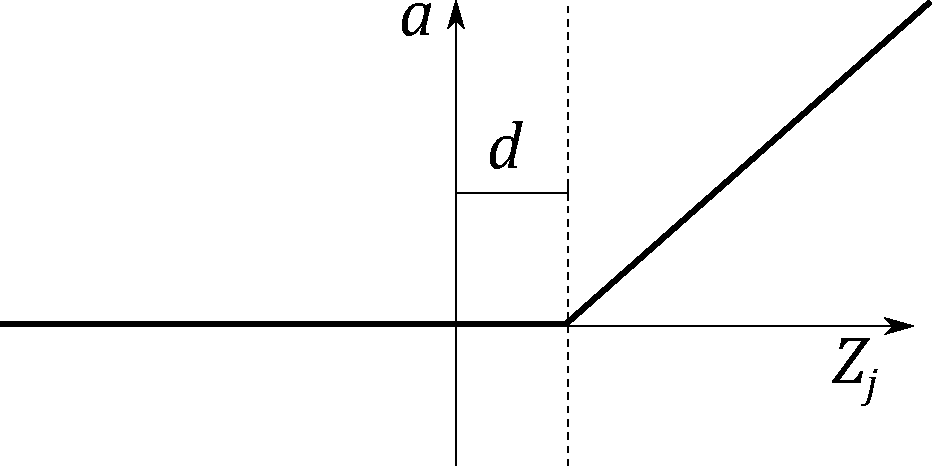
\includegraphics[width=0.5\linewidth]{images/relu.pdf}    

    \caption{In figure captions, explain what the reader is looking at: ``A schematic of the rectifying linear unit, where $a$ is the output amplitude,
    $d$ is a configurable dead-zone, and $Z_j$ is the input signal'', as well as why the reader is looking at this: 
    ``It is notable that there is no activation \emph{at all} below 0, which explains our initial results.'' 
    \textbf{Use vector image formats (.pdf) where possible}. Size figures appropriately, and do not make them over-large or too small to read.
    }

    % use the notation fig:name to cross reference a figure
    \label{fig:relu} 
\end{figure}


\begin{figure}
    \centering
    \begin{subfigure}[b]{0.45\textwidth}
        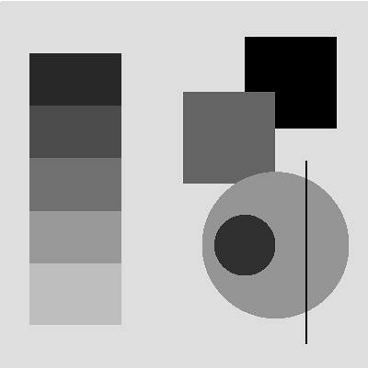
\includegraphics[width=\textwidth]{images/synthetic.png}
        \caption{Synthetic image, black on white.}
        \label{fig:syn1}
    \end{subfigure}
    ~ %add desired spacing between images, e. g. ~, \quad, \qquad, \hfill etc. 
      %(or a blank line to force the subfigure onto a new line)
    \begin{subfigure}[b]{0.45\textwidth}
        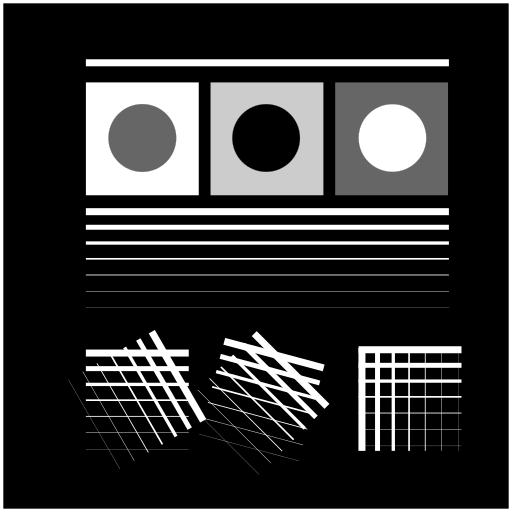
\includegraphics[width=\textwidth]{images/synthetic_2.png}
        \caption{Synthetic image, white on black.}
        \label{fig:syn2}
    \end{subfigure}
    ~ %add desired spacing between images, e. g. ~, \quad, \qquad, \hfill etc. 
    %(or a blank line to force the subfigure onto a new line)    
    \caption{Synthetic test images for edge detection algorithms. \subref{fig:syn1} shows various gray levels that require an adaptive algorithm. \subref{fig:syn2}
    shows more challenging edge detection tests that have crossing lines. Fusing these into full segments typically requires algorithms like the Hough transform.
    This is an example of using subfigures, with \texttt{subref}s in the caption.
    }\label{fig:synthetic}
\end{figure}

\clearpage

\subsection{Equations}

Equations should be typeset correctly and precisely. Make sure you get parenthesis sizing correct, and punctuate equations correctly 
(the comma is important and goes \textit{inside} the equation block). Explain any symbols used clearly if not defined earlier. 

For example, we might define:
\begin{equation}
    \hat{f}(\xi) = \frac{1}{2}\left[ \int_{-\infty}^{\infty} f(x) e^{2\pi i x \xi} \right],
\end{equation}    
where $\hat{f}(\xi)$ is the Fourier transform of the time domain signal $f(x)$.

\subsection{Algorithms}
Algorithms can be set using \texttt{algorithm2e}, as in Algorithm \ref{alg:metropolis}.

% NOTE: line ends are denoted by \; in algorithm2e
\begin{algorithm}
    \DontPrintSemicolon
    \KwData{$f_X(x)$, a probability density function returing the density at $x$.\; $\sigma$ a standard deviation specifying the spread of the proposal distribution.\;
    $x_0$, an initial starting condition.}
    \KwResult{$s=[x_1, x_2, \dots, x_n]$, $n$ samples approximately drawn from a distribution with PDF $f_X(x)$.}
    \Begin{
        $s \longleftarrow []$\;
        $p \longleftarrow f_X(x)$\;
        $i \longleftarrow 0$\;
        \While{$i < n$}
        {
            $x^\prime \longleftarrow \mathcal{N}(x, \sigma^2)$\;
            $p^\prime \longleftarrow f_X(x^\prime)$\;
            $a \longleftarrow \frac{p^\prime}{p}$\;
            $r \longleftarrow U(0,1)$\;
            \If{$r<a$}
            {
                $x \longleftarrow x^\prime$\;
                $p \longleftarrow f_X(x)$\;
                $i \longleftarrow i+1$\;
                append $x$ to $s$\;
            }
        }
    }
    
\caption{The Metropolis-Hastings MCMC algorithm for drawing samples from arbitrary probability distributions, 
specialised for normal proposal distributions $q(x^\prime|x) = \mathcal{N}(x, \sigma^2)$. The symmetry of the normal distribution means the acceptance rule takes the simplified form.}\label{alg:metropolis}
\end{algorithm}

\subsection{Tables}

If you need to include tables, like Table \ref{tab:operators}, use a tool like https://www.tablesgenerator.com/ to generate the table as it is
extremely tedious otherwise. 

\begin{table}[]
    \caption{The standard table of operators in Python, along with their functional equivalents from the \texttt{operator} package. Note that table
    captions go above the table, not below. Do not add additional rules/lines to tables. }\label{tab:operators}
    %\tt 
    \rowcolors{2}{}{gray!3}
    \begin{tabular}{@{}lll@{}}
    %\toprule
    \textbf{Operation}    & \textbf{Syntax}                & \textbf{Function}                            \\ %\midrule % optional rule for header
    Addition              & \texttt{a + b}                          & \texttt{add(a, b)}                                    \\
    Concatenation         & \texttt{seq1 + seq2}                    & \texttt{concat(seq1, seq2)}                           \\
    Containment Test      & \texttt{obj in seq}                     & \texttt{contains(seq, obj)}                           \\
    Division              & \texttt{a / b}                          & \texttt{div(a, b) }  \\
    Division              & \texttt{a / b}                          & \texttt{truediv(a, b) } \\
    Division              & \texttt{a // b}                         & \texttt{floordiv(a, b)}                               \\
    Bitwise And           & \texttt{a \& b}                         & \texttt{and\_(a, b)}                                  \\
    Bitwise Exclusive Or  & \texttt{a \textasciicircum b}           & \texttt{xor(a, b)}                                    \\
    Bitwise Inversion     & \texttt{$\sim$a}                        & \texttt{invert(a)}                                    \\
    Bitwise Or            & \texttt{a | b}                          & \texttt{or\_(a, b)}                                   \\
    Exponentiation        & \texttt{a ** b}                         & \texttt{pow(a, b)}                                    \\
    Identity              & \texttt{a is b}                         & \texttt{is\_(a, b)}                                   \\
    Identity              & \texttt{a is not b}                     & \texttt{is\_not(a, b)}                                \\
    Indexed Assignment    & \texttt{obj{[}k{]} = v}                 & \texttt{setitem(obj, k, v)}                           \\
    Indexed Deletion      & \texttt{del obj{[}k{]}}                 & \texttt{delitem(obj, k)}                              \\
    Indexing              & \texttt{obj{[}k{]}}                     & \texttt{getitem(obj, k)}                              \\
    Left Shift            & \texttt{a \textless{}\textless b}       & \texttt{lshift(a, b)}                                 \\
    Modulo                & \texttt{a \% b}                         & \texttt{mod(a, b)}                                    \\
    Multiplication        & \texttt{a * b}                          & \texttt{mul(a, b)}                                    \\
    Negation (Arithmetic) & \texttt{- a}                            & \texttt{neg(a)}                                       \\
    Negation (Logical)    & \texttt{not a}                          & \texttt{not\_(a)}                                     \\
    Positive              & \texttt{+ a}                            & \texttt{pos(a)}                                       \\
    Right Shift           & \texttt{a \textgreater{}\textgreater b} & \texttt{rshift(a, b)}                                 \\
    Sequence Repetition   & \texttt{seq * i}                        & \texttt{repeat(seq, i)}                               \\
    Slice Assignment      & \texttt{seq{[}i:j{]} = values}          & \texttt{setitem(seq, slice(i, j), values)}            \\
    Slice Deletion        & \texttt{del seq{[}i:j{]}}               & \texttt{delitem(seq, slice(i, j))}                    \\
    Slicing               & \texttt{seq{[}i:j{]}}                   & \texttt{getitem(seq, slice(i, j))}                    \\
    String Formatting     & \texttt{s \% obj}                       & \texttt{mod(s, obj)}                                  \\
    Subtraction           & \texttt{a - b}                          & \texttt{sub(a, b)}                                    \\
    Truth Test            & \texttt{obj}                            & \texttt{truth(obj)}                                   \\
    Ordering              & \texttt{a \textless b}                  & \texttt{lt(a, b)}                                     \\
    Ordering              & \texttt{a \textless{}= b}               & \texttt{le(a, b)}                                     \\
    % \bottomrule
    \end{tabular}
    \end{table}
\subsection{Code}

Avoid putting large blocks of code in the report (more than a page in one block, for example). Use syntax highlighting if possible, as in Listing \ref{lst:callahan}.

\begin{lstlisting}[language=python, float, caption={The algorithm for packing the $3\times 3$ outer-totalistic binary CA successor rule into a 
    $16\times 16\times 16\times 16$ 4 bit lookup table, running an equivalent, notionally 16-state $2\times 2$ CA.}, label=lst:callahan]
    def create_callahan_table(rule="b3s23"):
        """Generate the lookup table for the cells."""        
        s_table = np.zeros((16, 16, 16, 16), dtype=np.uint8)
        birth, survive = parse_rule(rule)

        # generate all 16 bit strings
        for iv in range(65536):
            bv = [(iv >> z) & 1 for z in range(16)]
            a, b, c, d, e, f, g, h, i, j, k, l, m, n, o, p = bv

            # compute next state of the inner 2x2
            nw = apply_rule(f, a, b, c, e, g, i, j, k)
            ne = apply_rule(g, b, c, d, f, h, j, k, l)
            sw = apply_rule(j, e, f, g, i, k, m, n, o)
            se = apply_rule(k, f, g, h, j, l, n, o, p)

            # compute the index of this 4x4
            nw_code = a | (b << 1) | (e << 2) | (f << 3)
            ne_code = c | (d << 1) | (g << 2) | (h << 3)
            sw_code = i | (j << 1) | (m << 2) | (n << 3)
            se_code = k | (l << 1) | (o << 2) | (p << 3)

            # compute the state for the 2x2
            next_code = nw | (ne << 1) | (sw << 2) | (se << 3)

            # get the 4x4 index, and write into the table
            s_table[nw_code, ne_code, sw_code, se_code] = next_code

        return s_table

\end{lstlisting}

%==================================================================================================================================
\chapter{Evaluation} 
How good is your solution? How well did you solve the general problem, and what evidence do you have to support that?

\section{Guidance}
\begin{itemize}
    \item
        Ask specific questions that address the general problem.
    \item
        Answer them with precise evidence (graphs, numbers, statistical
        analysis, qualitative analysis).
    \item
        Be fair and be scientific.
    \item
        The key thing is to show that you know how to evaluate your work, not
        that your work is the most amazing product ever.
\end{itemize}

\section{Evidence}
Make sure you present your evidence well. Use appropriate visualisations, reporting techniques and statistical analysis, as appropriate.

If you visualise, follow the basic rules, as illustrated in figure \ref{fig:boxplot}:
\begin{itemize}
\item Label everything correctly (axis, title, units).
\item Caption thoroughly.
\item Reference in text.
\item \textbf{Include appropriate display of uncertainty (e.g. error bars, Box plot)}
\item Minimize clutter.
\end{itemize}

See the file \texttt{guide\_to\_visualising.pdf} for further information and guidance.

\begin{figure}
    \centering
    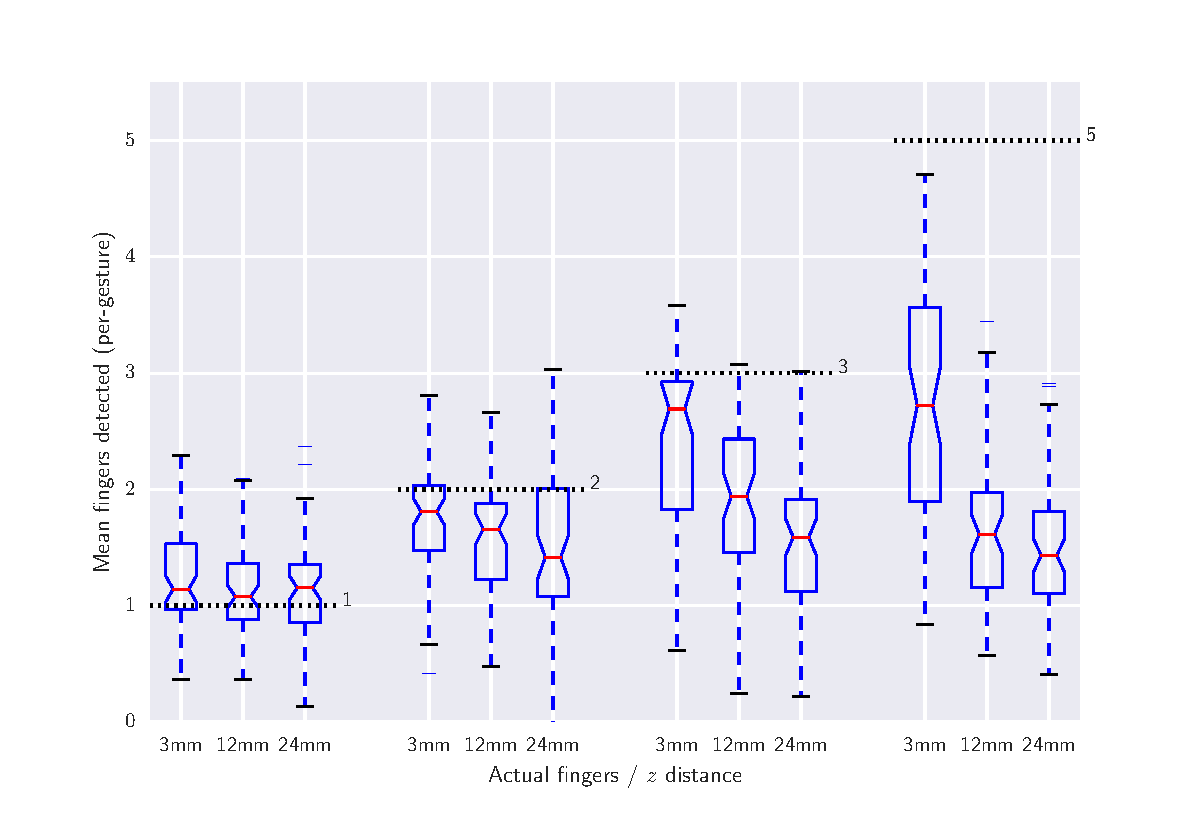
\includegraphics[width=1.0\linewidth]{images/boxplot_finger_distance.pdf}    

    \caption{Average number of fingers detected by the touch sensor at different heights above the surface, averaged over all gestures. Dashed lines indicate
    the true number of fingers present. The Box plots include bootstrapped uncertainty notches for the median. It is clear that the device is biased toward 
    undercounting fingers, particularly at higher $z$ distances.
    }

    % use the notation fig:name to cross reference a figure
    \label{fig:boxplot} 
\end{figure}


%==================================================================================================================================
\chapter{Conclusion}    
Summarise the whole project for a lazy reader who didn't read the rest (e.g. a prize-awarding committee).
\section{Guidance}
\begin{itemize}
    \item
        Summarise briefly and fairly.
    \item
        You should be addressing the general problem you introduced in the
        Introduction.        
    \item
        Include summary of concrete results (``the new compiler ran 2x
        faster'')
    \item
        Indicate what future work could be done, but remember: \textbf{you
        won't get credit for things you haven't done}.
\end{itemize}

%==================================================================================================================================
%
% 
%==================================================================================================================================
%  APPENDICES  

\begin{appendices}

\chapter{Appendices}

Typical inclusions in the appendices are:

\begin{itemize}
\item
  Copies of ethics approvals (required if obtained)
\item
  Copies of questionnaires etc. used to gather data from subjects.
\item
  Extensive tables or figures that are too bulky to fit in the main body of
  the report, particularly ones that are repetitive and summarised in the body.

\item Outline of the source code (e.g. directory structure), or other architecture documentation like class diagrams.

\item User manuals, and any guides to starting/running the software.

\end{itemize}

\textbf{Don't include your source code in the appendices}. It will be
submitted separately.

\end{appendices}

%==================================================================================================================================
%   BIBLIOGRAPHY   

% The bibliography style is abbrvnat
% The bibliography always appears last, after the appendices.

\bibliographystyle{unsrt}

\bibliography{l4proj}




\end{document}
